\chapter{CƠ SỞ LÝ THUYẾT}
\label{chap:cosolythuyet}

Chương này trình bày kiến thức nền về trí tuệ nhân tạo, học máy, học sâu, xử lý ảnh và biểu diễn đặc trưng. Nội dung tập trung vào cách mô hình học từ dữ liệu, cách thông tin ảnh được thu nhận, biến đổi và rút gọn. Mục cuối tổng hợp các nghiên cứu liên quan đến nhận diện biển báo. Bài toán, phương pháp áp dụng và cách đánh giá được trình bày ở Chương 2.

% Kiến thức nền; giữ các hình và bảng đang dùng trong báo cáo.
\section{Trí tuệ nhân tạo và thị giác máy tính}
\subsection{Khái niệm và mục tiêu của trí tuệ nhân tạo}
Trí tuệ nhân tạo (Artificial Intelligence -- AI) nghiên cứu cách xây dựng các hệ thống có khả năng nhận biết, suy luận, học từ dữ liệu và đưa ra quyết định trong một phạm vi nhiệm vụ xác định. Một hệ thống có thể hoạt động theo các quy tắc do con người thiết kế hoặc dùng mô hình được học từ các ví dụ~\cite{goodfellow2016deep}.

Trong nhận diện biển báo, thông tin ban đầu chỉ là các điểm ảnh. Hệ thống phải tìm được vùng chứa biển, phân biệt loại biển và đọc nội dung nếu có. Chẳng hạn, một vùng tròn màu đỏ có thể là biển giao thông nhưng cũng có thể là logo trên xe. Vì vậy, việc nhận diện cần kết hợp nhiều dấu hiệu thay vì chỉ kiểm tra một màu hoặc một hình dạng.

\subsection{Mối quan hệ giữa trí tuệ nhân tạo, học máy và học sâu}
Học máy (Machine Learning -- ML) là một nhánh của trí tuệ nhân tạo, trong đó mô hình học quy luật từ dữ liệu. Học sâu (Deep Learning -- DL) thuộc học máy và sử dụng mạng nơ-ron nhiều lớp để học cách biểu diễn dữ liệu. Như vậy, học sâu nằm trong học máy, còn học máy nằm trong trí tuệ nhân tạo. Mạng nơ-ron ít lớp cũng là mô hình học máy, nhưng thường không được gọi là mạng sâu~\cite{goodfellow2016deep}.

Có thể hình dung sự khác nhau qua ba cách nhận diện một vùng biển báo. Cách thứ nhất dùng quy tắc chọn vùng đỏ gần tròn. Cách thứ hai tính các đặc trưng màu, hình dạng rồi học một bộ phân loại từ những vùng đã gán nhãn. Cách thứ ba dùng mạng sâu để học đặc trưng trực tiếp từ ảnh. Hình~\ref{fig:ai_ml_dl} minh hoạ quan hệ này.

\begin{figure}[H]
\centering
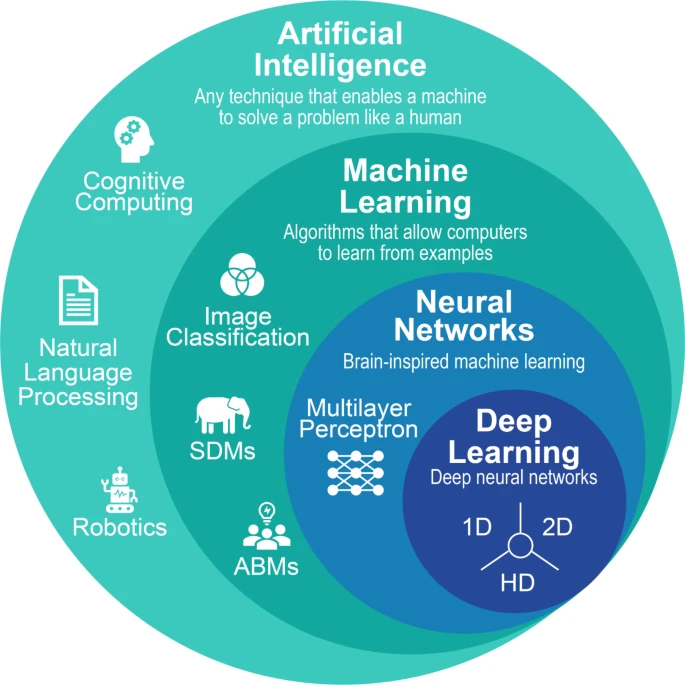
\includegraphics[width=.65\textwidth]{figures/sodoquanhe.png}
\caption[Mối quan hệ giữa AI, học máy, mạng nơ-ron và học sâu]{Mối quan hệ giữa trí tuệ nhân tạo, học máy, mạng nơ-ron và học sâu. }
\label{fig:ai_ml_dl}
\end{figure}

\subsection{Thị giác máy tính và các bài toán cơ bản}
Thị giác máy tính (Computer Vision) khai thác thông tin từ ảnh và video. Xử lý ảnh thường tạo ra một ảnh mới, chẳng hạn ảnh giảm nhiễu hoặc ảnh rõ tương phản hơn; thị giác máy tính dùng những thông tin đó để mô tả đối tượng và cảnh~\cite{tailieu_bai1}. Một hệ thống thị giác có thể sử dụng cả quy tắc xử lý ảnh, mô hình học máy và mạng sâu.

Các nhiệm vụ cơ bản gồm phân loại, phát hiện, phân đoạn và theo dõi. Phân loại trả lời đối tượng thuộc loại nào. Phát hiện còn xác định vị trí bằng khung bao. Phân đoạn xác định các điểm ảnh thuộc từng vùng. Theo dõi liên kết đối tượng qua nhiều khung hình~\cite{szeliski2022vision}. Với ảnh biển báo đã cắt sẵn, hệ thống chỉ cần phân loại vùng ảnh đó; với ảnh đường phố, hệ thống phải tìm biển giữa nhiều vật thể khác trước khi xác định lớp. Nhận dạng ký tự bổ sung bước chuyển chữ và số trong vùng biển thành văn bản.

\subsection{Quá trình thu nhận ảnh}
Ảnh số được tạo từ ánh sáng phản xạ trên vật thể đi qua hệ quang học và tới cảm biến. Lấy mẫu chia mặt phẳng ảnh thành các vị trí rời rạc; lượng tử hoá biểu diễn mức sáng tại mỗi vị trí bằng một tập giá trị hữu hạn. Đây là hai bước khác nhau: tăng số điểm ảnh làm lưới lấy mẫu dày hơn, còn tăng số bit làm các mức cường độ được biểu diễn chi tiết hơn~\cite{tailieu_bai1}.

Diện mạo của một vật trên ảnh phụ thuộc cả đặc điểm bề mặt lẫn nguồn sáng và cách ghi hình. Cùng một mặt biển màu đỏ có thể xuất hiện tối hơn trong bóng râm hoặc nhạt màu khi bị phản sáng. Khi vùng ảnh đã bão hoà trắng hoặc mất chi tiết trong vùng tối, thao tác tăng sáng sau đó không thể tạo lại những nét chưa được ghi nhận.

Chuyển động trong thời gian phơi sáng tạo vệt mờ, còn lấy nét không đúng làm các ranh giới bị trải rộng. Nén ảnh cũng có thể sinh các khối hoặc dao động quanh biên. Vì vậy, độ phân giải không phải tiêu chí duy nhất về chất lượng: một ảnh lớn nhưng mờ có thể chứa ít thông tin nhận dạng hơn một vùng ảnh nhỏ được lấy nét tốt.

\section{Học máy}
\subsection{Các hình thức học và quy trình xây dựng mô hình}
Các hình thức học được phân biệt theo thông tin dùng trong quá trình huấn luyện. Với học có giám sát, mỗi mẫu có nhãn đích, ví dụ ảnh và tên loại biển. Học không giám sát tìm cấu trúc trong dữ liệu chưa có nhãn, như nhóm các ảnh có đặc điểm gần nhau. Học bán giám sát kết hợp cả hai nguồn dữ liệu; một cách thực hiện là chọn các dự đoán đủ tin cậy làm nhãn giả để tiếp tục huấn luyện. Học tăng cường học cách hành động thông qua tương tác với môi trường và phần thưởng~\cite{google_intro_ml,google_ml_types}.

Bảng~\ref{tab:hinhthuchoc} và Hình~\ref{fig:machine_learning} tóm tắt bốn hình thức trên. Việc chọn hình thức học phụ thuộc nhiệm vụ và dữ liệu có sẵn. Phân loại biển từ ảnh có nhãn thường là bài toán có giám sát; phân cụm ảnh phục vụ kiểm tra dữ liệu là ví dụ của học không giám sát.

Một quy trình học máy bắt đầu từ xác định đầu vào và nhãn, kiểm tra dữ liệu, chọn biểu diễn, huấn luyện rồi đánh giá trên các mẫu độc lập. Chất lượng nhãn và cách chia dữ liệu ảnh hưởng trực tiếp đến độ tin cậy của kết quả, ngay cả khi thuật toán được giữ nguyên.

\begin{table}[H]
\centering
\caption[Các hình thức học máy cơ bản]{Các hình thức học máy cơ bản; tổng hợp theo~\cite{google_intro_ml,google_ml_types}.}
\label{tab:hinhthuchoc}
\small
\begin{tabularx}{\textwidth}{|>{\raggedright\arraybackslash}p{2.5cm}|>{\raggedright\arraybackslash}X|>{\raggedright\arraybackslash}X|}
\toprule
\textbf{Hình thức học} & \textbf{Dữ liệu và cách học} & \textbf{Kết quả và ví dụ dễ hình dung} \\
\midrule
Học có giám sát & Dữ liệu có nhãn đúng. Mô hình so sánh dự đoán với nhãn để điều chỉnh tham số. & Dự đoán lớp hoặc giá trị: học từ ảnh đã ghi nhãn để phân loại biển cấm, biển nguy hiểm. \\ \hline
Học không giám sát & Dữ liệu không có nhãn. Mô hình tìm cấu trúc, sự tương đồng hoặc cách biểu diễn gọn hơn. & Phân cụm hoặc giảm chiều: nhóm ảnh biển báo có đặc điểm tương tự để hỗ trợ khám phá dữ liệu. \\ \hline
Học bán giám sát & Kết hợp dữ liệu có nhãn với dữ liệu chưa gán nhãn; có thể dùng nhãn giả được chọn lọc. & Tận dụng ảnh chưa gán nhãn để hỗ trợ huấn luyện; cần kiểm soát nhãn giả sai. \\ \hline
Học tăng cường & Tác nhân thực hiện hành động, nhận thưởng hoặc phạt từ môi trường và học qua tương tác. & Học chính sách tối đa hoá tổng phần thưởng, ví dụ điều khiển xe trong mô phỏng. \\
\bottomrule
\end{tabularx}
\end{table}


\begin{figure}[H]
\centering
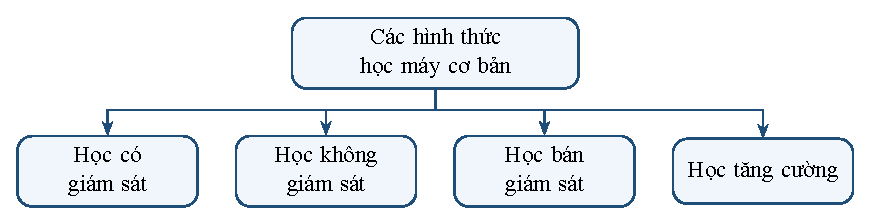
\includegraphics[width=.9\textwidth]{figures/fig_1_2_learning_methods.pdf}
\caption[Các hình thức học máy cơ bản]{Các hình thức học máy cơ bản}
\label{fig:machine_learning}
\end{figure}

\subsection{Các mô hình học máy}
Các mô hình học máy thường nhận một vector đặc trưng và trả về lớp hoặc điểm dự đoán. Màu sắc, hình dạng và cấu trúc nét là những nguồn thông tin có thể đưa vào vector; cách biểu diễn và giảm chiều được trình bày tại Mục~\ref{sec:image_features}.

Máy vector hỗ trợ (Support Vector Machine -- SVM) học ranh giới phân chia các nhóm mẫu với biên phân cách lớn. Các mẫu gần ranh giới có vai trò quyết định cách đặt biên; hàm kernel cho phép xây dựng ranh giới phi tuyến~\cite{cortes1995svm,sklearn_svm}. Với một số mẫu khó, mô hình có thể chấp nhận sai số để cân bằng giữa biên phân cách rộng và mức khớp dữ liệu. Một đặc trưng có giá trị lớn chỉ vì đơn vị đo cũng có thể chi phối khoảng cách, nên cần xem xét chuẩn hoá đầu vào.

Cây quyết định tách dữ liệu bằng những câu hỏi theo đặc trưng, ví dụ tỉ lệ màu có vượt một ngưỡng hay không. Một cây sâu có thể mô tả nhiều trường hợp riêng nhưng dễ phụ thuộc nhiễu. Rừng ngẫu nhiên (Random Forest) tổng hợp dự đoán của nhiều cây được học với sự ngẫu nhiên trong lựa chọn mẫu và đặc trưng. Nhờ đó, kết quả ít phụ thuộc vào một cây đơn lẻ~\cite{sklearn_ensemble}.

LightGBM thuộc nhóm tăng cường cây: các cây được bổ sung theo từng bước để giảm sai số còn lại. Khác với việc tổng hợp nhiều cây học tương đối độc lập, cây mới trong quá trình tăng cường được xây dựng dựa trên thông tin của mô hình hiện tại. Cơ chế chia các giá trị thành những khoảng rời rạc giúp tìm phép tách hiệu quả hơn về thời gian và bộ nhớ~\cite{ke2017lightgbm,lightgbm_features}. Số cây, số lá và tốc độ học ảnh hưởng đến độ phức tạp; tăng các giá trị này không tự bảo đảm dự đoán tốt hơn trên ảnh mới.

Đầu ra của bộ phân loại có thể là nhãn, điểm quyết định hoặc một giá trị biểu diễn mức tin cậy. Các giá trị cùng nằm trong khoảng từ 0 đến 1 chưa chắc đã có cùng ý nghĩa xác suất. Chẳng hạn, trong nhóm mẫu được gán điểm gần $0{,}8$ cho một sự kiện, tỉ lệ sự kiện đó thực sự xảy ra có thể thấp hơn mức này. Hiệu chỉnh điểm dự đoán dùng dữ liệu thích hợp để kiểm tra và điều chỉnh quan hệ đó; nó khác với việc chỉ chọn một ngưỡng chấp nhận~\cite{sklearn_calibration}.

\subsection{Chia dữ liệu, quá khớp và khả năng tổng quát hoá}
Tập huấn luyện được dùng để học tham số. Tập xác thực dùng để lựa chọn mô hình, siêu tham số và ngưỡng quyết định. Tập kiểm thử dùng để đánh giá sau khi các lựa chọn đã được chốt. Những bước học từ dữ liệu như chuẩn hoá hoặc PCA chỉ được khớp trên phần huấn luyện thích hợp, sau đó mới áp dụng sang các tập còn lại~\cite{sklearn_pitfalls}.

Quá khớp xảy ra khi mô hình học quá sát các chi tiết riêng của tập huấn luyện và dự đoán kém trên mẫu mới. Một dấu hiệu thường gặp là sai số huấn luyện tiếp tục giảm nhưng chất lượng xác thực giảm hoặc không cải thiện. Giới hạn độ phức tạp, tăng cường dữ liệu phù hợp và dừng sớm có thể giảm hiện tượng này. Nếu chất lượng trên cả hai tập đều thấp, cần xem lại khả năng biểu diễn, dữ liệu và quá trình huấn luyện.

Ảnh lấy từ cùng một đoạn video có thể gần như trùng nhau. Chia ngẫu nhiên từng ảnh dễ đưa các cảnh rất giống nhau vào cả tập học và tập kiểm thử. Chia theo video, phiên ghi hình hoặc cụm ảnh gần trùng sẽ hạn chế nguy cơ này. Với hệ thống có nhiều mô hình, dữ liệu dùng để huấn luyện bất kỳ thành phần nào đều phải tách khỏi tập kiểm thử của toàn hệ thống.

\section{Mạng nơ-ron và học sâu}
\subsection{Mạng nơ-ron nhân tạo và mạng tích chập}
Một nơ-ron nhân tạo nhận các giá trị đầu vào, tính tổng có trọng số, cộng độ lệch rồi đưa qua hàm kích hoạt. Với đầu vào $\mathbf{x}$, trọng số $\mathbf{w}$ và độ lệch $b$, đầu ra là:
\begin{equation}
 y=\phi(\mathbf{w}^{\top}\mathbf{x}+b).
 \label{eq:neuron}
\end{equation}
Hàm $\phi$ tạo tính phi tuyến; ví dụ ReLU có dạng $\phi(z)=\max(0,z)$. Nhiều lớp nơ-ron kết hợp các biểu diễn trung gian để mô tả quan hệ phức tạp hơn giữa đầu vào và đầu ra~\cite{stanford_neuralnets}.

Mạng nơ-ron tích chập (Convolutional Neural Network -- CNN) xử lý ảnh bằng các bộ lọc nhỏ dùng chung trọng số tại nhiều vị trí. Một bộ lọc có thể phản ứng với nét ngang, nét dọc hoặc một mẫu cục bộ. Với đầu vào một kênh $X$, bộ lọc $K$ kích thước $k\times k$, bước trượt bằng 1 và bỏ qua xử lý biên, ta có:
\begin{equation}
 Y(i,j)=\phi\!\left(b+\sum_{u=0}^{k-1}\sum_{v=0}^{k-1}K(u,v)X(i+u,j+v)\right).
 \label{eq:conv}
\end{equation}
Trong đó $Y(i,j)$ là giá trị đầu ra tại vị trí $(i,j)$; $u,v$ là chỉ số trong bộ lọc. Với đầu vào nhiều kênh, phép tính còn cộng theo các kênh đó. Trong các thư viện học sâu, thao tác này thường gọi là tích chập dù được thực hiện theo dạng tương quan chéo.

Các lớp đầu học những mẫu cục bộ; các lớp sau kết hợp chúng thành biểu diễn rộng hơn. Bước trượt và phần đệm điều chỉnh kích thước bản đồ đặc trưng. Lớp gộp làm giảm độ phân giải, giúp giảm tính toán nhưng cũng có thể làm mất chi tiết của đối tượng nhỏ~\cite{stanford_cs231n_cnn}. Hình~\ref{fig:cnn} minh hoạ một mạng phân loại gồm phần trích đặc trưng và phần đưa ra lớp dự đoán; những kiến trúc khác có thể thay đổi cách tổ chức đầu ra.

Vùng tiếp nhận của một giá trị đặc trưng là phần ảnh đầu vào có thể ảnh hưởng đến nó. Khi đi qua nhiều lớp tích chập và giảm kích thước, vùng tiếp nhận thường mở rộng. Nhờ vậy, các lớp sâu có thể kết hợp nét cục bộ với hình dạng rộng hơn. Tuy nhiên, vùng tiếp nhận lớn không bảo đảm giữ được chi tiết nhỏ nếu chi tiết đã mất trong các bước giảm độ phân giải.

Việc dùng chung bộ lọc giúp CNN nhận ra một mẫu tại nhiều vị trí mà không cần học một bộ trọng số riêng cho từng điểm ảnh. Khả năng này khác với bất biến hoàn toàn trước mọi phép biến đổi. Đổi tỉ lệ, xoay mạnh, thay ánh sáng hoặc che khuất vẫn có thể làm biểu diễn và dự đoán thay đổi. Dữ liệu huấn luyện cần phản ánh những biến đổi có ý nghĩa đối với nhiệm vụ~\cite{stanford_cs231n_cnn}.

Các đầu ra phân loại thường tổng hợp đặc trưng của toàn vùng ảnh. Đầu ra phát hiện còn cần giữ thông tin về vị trí. Do đó, một vector đặc trưng dùng để phân loại ảnh đã cắt không thể được hiểu như danh sách vị trí đối tượng trên cả ảnh; hai kiểu đầu ra đòi hỏi cách tổ chức phần dự đoán khác nhau.

\begin{figure}[H]
\centering
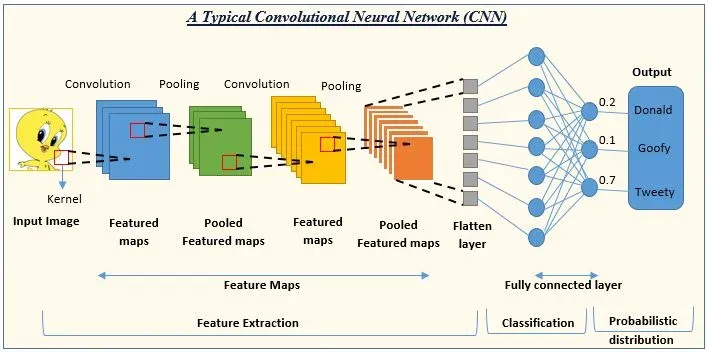
\includegraphics[width=.9\textwidth]{figures/Thuat-toan-CNN-co-cau-truc-nhu-the-nao.png}
\caption[Kiến trúc CNN cơ bản]{Mạng Neural tích chập(CNN) điển hình. nguồn ảnh: InterData~\cite{interdata_cnn_image}.}
\label{fig:cnn}
\end{figure}

\begin{table}[H]
\centering
\caption[So sánh học máy truyền thống và học sâu]{So sánh học máy truyền thống và học sâu trong xử lý ảnh.}
\label{tab:mldl}
\small
\begin{tabularx}{\textwidth}{|>{\raggedright\arraybackslash}p{2.5cm}|>{\raggedright\arraybackslash}X|>{\raggedright\arraybackslash}X|}
\toprule
\textbf{Tiêu chí} & \textbf{Học máy truyền thống} & \textbf{Học sâu} \\
\midrule
Luồng xử lý ảnh & Trích màu, biên, hình dạng hoặc HOG trước; đưa vector đặc trưng vào bộ phân loại. & Mạng nhiều lớp tự học đặc trưng và ánh xạ từ ảnh đến kết quả dự đoán. \\ \hline
Mô hình tiêu biểu & SVM, Random Forest, LightGBM. & CNN; mạng phát hiện đối tượng như YOLO. \\ \hline
Dữ liệu huấn luyện & Thường phù hợp với dữ liệu vừa hoặc nhỏ nếu đặc trưng được chọn tốt. & Huấn luyện từ đầu thường cần nhiều dữ liệu; học chuyển giao giúp giảm nhu cầu này. \\ \hline
Tài nguyên tính toán & Thường nhẹ hơn với vector đặc trưng gọn; nhiều mô hình huấn luyện được trên CPU. & Huấn luyện thường cần GPU; chi phí suy luận phụ thuộc kiến trúc và kích thước ảnh. \\ \hline
Ưu điểm và hạn chế & Dễ kiểm tra đặc trưng; hiệu quả phụ thuộc bước trích chọn, khó bao quát cảnh phức tạp. & Học được đặc trưng phức tạp; cần kiểm soát quá khớp và khó giải thích hơn. \\ \hline
Ví dụ ứng dụng & Kiểm tra vùng nghi ngờ bằng màu, hình dạng và các đặc trưng đã trích xuất. & Phát hiện, phân loại biển báo hoặc nhận dạng chữ trong vùng ảnh. \\
\bottomrule
\end{tabularx}
\end{table}


\subsection{Nguyên lý học của mạng nơ-ron}
Huấn luyện điều chỉnh tham số để giảm hàm mất mát, tức đại lượng đo sai khác giữa dự đoán và nhãn. Lan truyền ngược tính gradient của mất mát theo tham số; thuật toán tối ưu dùng thông tin đó để cập nhật mô hình. Dạng cập nhật cơ bản trên một lô nhỏ dữ liệu là:
\begin{equation}
 \theta_{t+1}=\theta_t-\eta\nabla_{\theta}\mathcal{L}_{\mathcal{B}_t}(\theta_t),
 \label{eq:gradient_update}
\end{equation}
với $\theta_t$ là tham số ở bước $t$, $\eta$ là tốc độ học và $\mathcal{L}_{\mathcal{B}_t}$ là mất mát trên lô $\mathcal{B}_t$. Một lượt đi qua toàn bộ tập huấn luyện được gọi là một epoch. Tốc độ học quá lớn có thể làm quá trình học dao động; tốc độ quá nhỏ làm cập nhật chậm~\cite{goodfellow_optimization}.

Học chuyển giao sử dụng biểu diễn đã học trên dữ liệu nguồn cho một nhiệm vụ mới. Có thể giữ cố định bộ trích đặc trưng và chỉ học phần dự đoán mới, hoặc tiếp tục cập nhật một phần hay toàn bộ mạng. Cách tiếp tục cập nhật này gọi là tinh chỉnh mô hình, hay fine-tuning~\cite{stanford_transfer}.

Với dữ liệu ảnh hạn chế, mô hình huấn luyện trước cung cấp các đặc trưng khởi đầu về biên, màu và kết cấu. Dữ liệu đích vẫn cần đủ đại diện cho điều kiện sử dụng, vì trọng số huấn luyện trước không thay thế được những ví dụ về biển nhỏ, ảnh mờ hoặc ban đêm. Bảng~\ref{tab:mldl} so sánh cách học từ đặc trưng thiết kế trước với cách học biểu diễn bằng mạng sâu.

Trong một lần học có giám sát, hàm mất mát đo sai khác giữa dự đoán và nhãn trên tập mẫu. Với phân loại, sai khác liên quan đến lớp dự đoán; với xác định vị trí, sai khác còn liên quan đến khung bao. Lựa chọn hàm mất mát phải phù hợp đầu ra cần học, trong khi chỉ số đánh giá phản ánh chất lượng theo tiêu chí sử dụng. Mất mát giảm không có nghĩa mọi nhóm lỗi đều giảm như nhau.

Các biện pháp giảm quá khớp có thể tác động vào dữ liệu hoặc mô hình. Tăng cường dữ liệu tạo thêm các biến đổi vẫn giữ được nhãn; giới hạn trọng số hoặc độ phức tạp hạn chế mô hình học những trường hợp quá riêng; dừng sớm chọn thời điểm trước khi chất lượng xác thực suy giảm. Một phép biến đổi làm đổi ý nghĩa đối tượng không còn là tăng cường giữ nguyên nhãn. Ví dụ, lật ngang một ký hiệu có hướng có thể tạo ra một lớp khác.

Khi học chuyển giao, mức khác biệt giữa dữ liệu nguồn và dữ liệu đích ảnh hưởng đến phần mạng nên được điều chỉnh. Giữ cố định nhiều lớp giảm số tham số cần học nhưng cũng hạn chế thích nghi. Cập nhật toàn bộ mạng cho phép thích nghi rộng hơn, đổi lại cần kiểm soát tốc độ học và mức quá khớp. Việc lựa chọn cần dựa trên dữ liệu xác thực, không chỉ dựa vào số lượng lớp của mô hình~\cite{stanford_transfer}.

\subsection{Các phương pháp phát hiện đối tượng}
Phát hiện đối tượng kết hợp phân loại với xác định vị trí. Hai hướng thường gặp là phát hiện hai giai đoạn và một giai đoạn, cũng được giới thiệu trong Bài 9 của tài liệu học phần~\cite{tailieu_bai9}.

Với hướng hai giai đoạn, Faster R-CNN dùng mạng đề xuất vùng để tìm những vị trí có khả năng chứa đối tượng. Đặc trưng ở các vùng này được dùng để phân loại và hiệu chỉnh khung bao. Mạng đề xuất vùng chia sẻ đặc trưng tích chập với mạng phát hiện, giảm việc trích đặc trưng lặp lại~\cite{ren2015faster}.

Với hướng một giai đoạn, các mô hình như YOLO dự đoán khung bao và thông tin lớp trực tiếp từ đặc trưng của ảnh. Cách tổ chức này phù hợp với những ứng dụng cần xử lý liên tiếp nhiều khung hình~\cite{redmon2016yolo,sapkota2025yolo}. Các phiên bản YOLO thay đổi về cấu trúc và cách huấn luyện; cấu trúc lưới của phiên bản đầu không phải mô tả chung cho mọi phiên bản sau.

Kết quả của hai hướng phụ thuộc dữ liệu, kích thước đầu vào, biến thể mạng và phần cứng. Với biển báo nhỏ, việc giảm độ phân giải có thể làm mất những nét giúp phân biệt lớp. Vì vậy cần xem xét đồng thời khả năng định vị, phân loại và thời gian xử lý khi lựa chọn mô hình.

\section{Xử lý ảnh số}
\subsection{Biểu diễn ảnh và các không gian màu}
Ảnh số là một lưới điểm ảnh. Ảnh xám lưu một giá trị cường độ tại mỗi điểm, còn ảnh RGB lưu ba thành phần đỏ, lục và lam. Với ảnh 8 bit mỗi kênh, giá trị thường nằm từ 0 đến 255~\cite{tailieu_bai1}. OpenCV thường đọc ảnh theo thứ tự kênh BGR, nên cần thống nhất thứ tự kênh trước khi hiển thị hoặc đưa ảnh vào mô hình.

HSV mô tả màu bằng sắc màu $H$, độ bão hoà $S$ và độ sáng $V$. Cách tách này thuận tiện để chọn vùng có màu gần nhau. Sắc màu có tính tuần hoàn, vì vậy vùng đỏ có thể nằm ở cả hai đầu miền giá trị $H$. Lab tách độ sáng $L^*$ khỏi hai trục màu: $a^*$ theo hướng lục--đỏ và $b^*$ theo hướng lam--vàng~\cite{opencv_color}. Xử lý riêng độ sáng có thể hạn chế thay đổi màu khi tăng tương phản.

Bảng~\ref{tab:khonggianmau} tóm tắt đặc điểm của từng không gian màu. Trong Hình~\ref{fig:color_spaces}, các kênh được hiển thị riêng bằng thang xám để quan sát giá trị: vùng sáng biểu thị giá trị kênh cao hơn, vùng tối biểu thị giá trị thấp hơn. Đây là cách xem từng kênh, không phải hiện tượng ảnh bị mất màu sau chuyển đổi. Riêng kênh sắc màu, giá trị cao hơn không có nghĩa là màu gốc sáng hơn.

\begin{table}[H]
\centering
\caption{Đặc điểm và vai trò của các không gian màu.}
\label{tab:khonggianmau}
\small
\begin{tabularx}{\textwidth}{|p{2.2cm}|p{3cm}|X|}
\toprule
\textbf{Không gian màu} & \textbf{Các thành phần} & \textbf{Vai trò trong xử lý ảnh} \\
\midrule
RGB & Đỏ, lục, lam & Biểu diễn ảnh màu và hiển thị kết quả \\ \hline
HSV & Sắc màu, độ bão hoà, độ sáng & Tạo mặt nạ vùng màu; phân tích màu đặc trưng của biển \\ \hline
Lab & Độ sáng L và hai thành phần màu a, b & Xử lý độ sáng, tương phản trên kênh L \\
\bottomrule
\end{tabularx}
\end{table}


\begin{figure}[H]
\centering
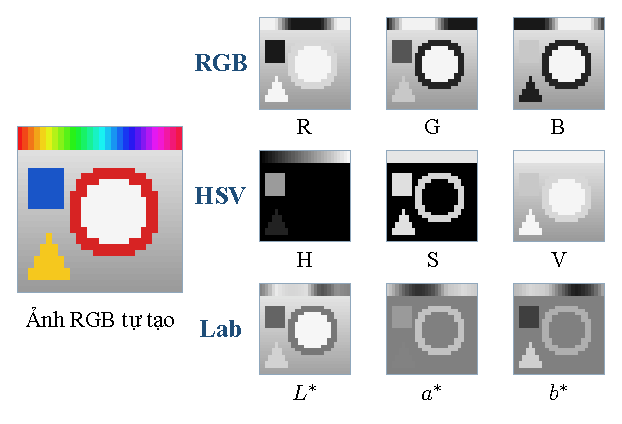
\includegraphics[width=.94\textwidth]{figures/fig_1_4_color_spaces.pdf}
\caption[Minh hoạ các kênh RGB, HSV và Lab]{Minh hoạ các kênh RGB, HSV và Lab . Giá trị các kênh được chuẩn hoá để hiển thị ở thang xám.}
\label{fig:color_spaces}
\end{figure}

\subsection{Lấy mẫu, đổi kích thước và cắt vùng ảnh}
Đổi kích thước ảnh tạo một lưới điểm ảnh mới. Giá trị ở vị trí mới được ước lượng từ các điểm ảnh cũ bằng nội suy. Nội suy láng giềng gần nhất lấy giá trị của điểm gần nhất; nội suy song tuyến tính kết hợp các điểm lân cận; các cách nội suy khác sử dụng vùng rộng hơn hoặc quan hệ diện tích khi thu nhỏ~\cite{opencv_geometry}.

Thu nhỏ làm giảm số điểm biểu diễn đối tượng. Nếu một nét chữ chỉ rộng vài điểm ảnh, nó có thể bị trộn với nền rồi biến mất. Khi phóng to, lưới mới dày hơn nhưng không bổ sung được thông tin chi tiết vốn không có trong ảnh gốc. Vì vậy, kích thước ảnh sau nội suy và lượng thông tin thực còn lại là hai vấn đề cần phân biệt.

Nếu ép một ảnh chữ nhật thành hình vuông bằng hai hệ số co giãn khác nhau, hình tròn có thể thành elip và tỉ lệ nét bị thay đổi. Giữ nguyên tỉ lệ rồi thêm phần đệm tránh biến dạng đó, nhưng phải lưu hệ số tỉ lệ và độ lệch do phần đệm để đổi toạ độ trở lại ảnh ban đầu. Lựa chọn này ảnh hưởng đến cả khung bao và vùng cắt dùng cho các bước sau.

Cắt vùng ảnh giữ lại một phần không gian cần quan sát. Vùng cắt quá hẹp có thể mất viền hoặc ký tự; vùng quá rộng đưa thêm nền và những vật thể khác vào bộ nhận dạng. Với ảnh nhị phân hoặc mặt nạ nhãn, nội suy cũng cần được chọn cẩn thận vì một phép nội suy tạo giá trị trung gian có thể làm thay đổi ý nghĩa của nhãn. Đây là lý do xử lý ảnh màu và xử lý mặt nạ không nhất thiết dùng cùng một phép nội suy.

\subsection{Chất lượng ảnh và điều chỉnh độ sáng}
Độ sáng, tương phản, nhiễu và độ mờ ảnh hưởng đến khả năng quan sát viền và nét chữ. Độ sáng trung bình phản ánh mức sáng chung; độ phân tán cường độ gợi ý mức tương phản. Phương sai đáp ứng Laplacian thường được dùng như một dấu hiệu về độ nét, nhưng nhiễu và nền nhiều chi tiết cũng làm đại lượng này tăng. Các chỉ báo cần được kết hợp và kiểm tra theo loại ảnh sử dụng.

Biến đổi gamma điều chỉnh cường độ để làm sáng hoặc tối ảnh. Cân bằng histogram thích nghi có giới hạn tương phản, thường gọi là CLAHE, thực hiện theo các vùng cục bộ và giới hạn mức tăng tương phản để giảm khuếch đại nhiễu~\cite{zuiderveld1994clahe,opencv_clahe}. Khi thao tác trên kênh độ sáng, màu của ảnh thường ít bị ảnh hưởng hơn so với xử lý độc lập từng kênh RGB.

Histogram là thống kê số điểm ảnh tại từng mức cường độ. Histogram tập trung trong một khoảng hẹp có thể gợi ý tương phản thấp, nhưng không cho biết các điểm sáng và tối nằm ở đâu. Hai ảnh có cách bố trí vật thể khác nhau vẫn có thể có histogram giống nhau. Vì vậy, thống kê toàn ảnh cần được xem cùng cấu trúc cục bộ và nội dung cần nhận dạng.

Với cường độ đã chuẩn hoá $r\in[0,1]$, một cách viết biến đổi gamma là:
\begin{equation}
 s=r^{1/\gamma},\qquad \gamma>0.
 \label{eq:gamma_intensity}
\end{equation}
Trong công thức này, $s$ là đầu ra, $\gamma>1$ làm tăng các mức sáng trung gian và $0<\gamma<1$ làm chúng tối hơn. Cần nêu rõ quy ước vì một số tài liệu viết số mũ trực tiếp là $\gamma$, khi đó chiều tác động của tham số được đảo lại. Hai đầu 0 và 1 vẫn được giữ nguyên.

Cân bằng histogram toàn ảnh dùng một phép biến đổi chung cho mọi vị trí. Với ảnh có vùng sáng và vùng tối khác nhau, tăng tương phản theo vùng có thể phù hợp hơn. CLAHE chia ảnh thành các vùng cục bộ, giới hạn histogram trước khi cân bằng và kết hợp kết quả giữa các vùng để giảm ranh giới giả~\cite{opencv_clahe}. Tăng tương phản cần giữ được các nét thật thay vì chỉ làm mọi chi tiết, kể cả nhiễu, nổi rõ hơn.

\subsection{Lọc nhiễu và làm nổi biên}
Phép lọc xét một vùng lân cận thay vì xử lý độc lập từng điểm ảnh. Lọc trung bình thay một điểm bằng trung bình các điểm quanh nó, nên làm giảm dao động nhưng cũng làm mờ ranh giới. Lọc Gaussian dùng trọng số lớn hơn cho các điểm gần tâm. Khi cửa sổ lọc hoặc độ trải Gaussian tăng, ảnh được làm trơn mạnh hơn và những cấu trúc nhỏ dễ bị mất~\cite{tomasi1998bilateral,opencv_filtering}.

Lọc trung vị sắp các giá trị trong cửa sổ và chọn giá trị ở giữa, phù hợp khi xuất hiện những điểm sáng hoặc tối bất thường rời rạc. Lọc song phương lại xét cả khoảng cách trên ảnh và khác biệt cường độ: hai điểm ở gần nhưng khác màu mạnh có thể được gán mức ảnh hưởng thấp. Nhờ đó một số ranh giới được giữ rõ hơn, nhưng chi phí tính toán và mức lọc vẫn phụ thuộc tham số.

\begin{table}[H]
\centering
\caption{Đặc điểm của một số phép lọc ảnh.}
\label{tab:filters_theory}
\small
\begin{tabularx}{\textwidth}{|>{\raggedright\arraybackslash}p{2.4cm}|>{\raggedright\arraybackslash}X|>{\raggedright\arraybackslash}X|}
\toprule
\textbf{Phép lọc} & \textbf{Cách xử lý} & \textbf{Điểm cần lưu ý} \\
\midrule
Gaussian & Lấy tổng có trọng số theo khoảng cách quanh tâm. & Giảm biến thiên nhỏ nhưng có thể làm mờ biên và nét chữ. \\ \hline
Trung vị & Chọn giá trị giữa trong cửa sổ. & Hữu ích với nhiễu xung; cửa sổ lớn có thể xoá nét mảnh. \\ \hline
Song phương & Kết hợp khoảng cách không gian và khác biệt cường độ. & Có thể giữ biên tốt hơn khi lọc; cần cân nhắc tham số và thời gian. \\
\bottomrule
\end{tabularx}
\end{table}

Đạo hàm ảnh mô tả mức thay đổi cường độ. Với ảnh xám $I$, hai đáp ứng theo chiều ngang và dọc được ký hiệu là $G_x,G_y$. Độ lớn và hướng biến thiên có thể tính bằng:
\begin{equation}
 m=\sqrt{G_x^2+G_y^2},\qquad
 \alpha=\operatorname{atan2}(G_y,G_x).
 \label{eq:gradient_magnitude}
\end{equation}
Độ lớn $m$ phản ánh mức thay đổi tại vị trí xét; góc $\alpha$ chỉ hướng tăng cường độ mạnh nhất, không phải hướng của đường biên. Những toán tử như Sobel ước lượng đạo hàm trên lưới ảnh; Laplacian sử dụng đạo hàm bậc hai để làm nổi những thay đổi cục bộ~\cite{opencv_gradients}.

Biên thật, nhiễu và các vân nền đều có thể tạo đáp ứng đạo hàm lớn. Lọc trước khi tính biên thường giúp giảm ảnh hưởng của nhiễu nhưng có thể làm yếu nét nhỏ. Đáp ứng có dấu cũng cần được lưu bằng kiểu số phù hợp; chuyển ngay sang số nguyên không dấu có thể làm mất phần âm. Kết quả tính biên là thông tin để mô tả hoặc phân vùng, chưa phải kết luận đối tượng thuộc lớp nào.

\subsection{Phân vùng ảnh và đặc trưng hình dạng}
Phân vùng ảnh tách các điểm ảnh thành những vùng có ý nghĩa, chẳng hạn mặt nạ vùng đỏ hoặc vùng sáng chứa chữ. Ngưỡng theo màu là cách thực hiện đơn giản, nhưng nhạy với ánh sáng và bóng đổ. Phát hiện biên tìm nơi cường độ biến đổi mạnh; đường bao mô tả ranh giới của một vùng. Một ảnh biên có thể chứa nhiều đoạn rời, chưa tạo thành đường bao hoàn chỉnh của đối tượng.

Các phép hình thái học dùng phần tử cấu trúc, tức một mẫu lân cận nhỏ, để điều chỉnh hình dạng vùng. Trên ảnh nhị phân có tiền cảnh trắng, phép co làm thu hẹp vùng trắng, phép giãn làm mở rộng vùng trắng. Phép mở là co rồi giãn, thường loại đốm nhỏ; phép đóng là giãn rồi co, có thể lấp lỗ nhỏ hoặc khe hẹp~\cite{opencv_morphology}. Kích thước phần tử cấu trúc cần phù hợp với chi tiết muốn giữ.

Hàng trên của Hình~\ref{fig:morphology_shapes} minh hoạ bốn phép xử lý với cùng một ảnh nhị phân. Hàng dưới là các hình học độc lập để minh hoạ đặc trưng: nét đỏ chỉ đường bao, nét xanh đứt chỉ khung chữ nhật bao quanh, chấm đen chỉ tâm. Hình tròn, tam giác và hình vuông xoay nghiêng không phải kết quả của các phép xử lý ở hàng trên.

Từ đường bao có thể tính diện tích, chu vi, tâm và số đỉnh sau xấp xỉ đa giác~\cite{opencv_contours}. Độ tròn là một ví dụ:
\begin{equation}
 C=\frac{4\pi A}{P^2},
 \label{eq:circularity}
\end{equation}
trong đó $A$ là diện tích, $P$ là chu vi. Hình tròn lý tưởng có $C=1$; những hình kém tròn có giá trị nhỏ hơn. Trên ảnh số, cách lấy đường bao ảnh hưởng đến kết quả. Tỉ lệ rộng/cao, độ đặc (diện tích vùng chia cho diện tích bao lồi) và số đỉnh bổ sung thông tin về hình dạng. Góc nhìn nghiêng có thể làm biển tròn xuất hiện thành elip, nên cần kết hợp các đặc trưng thay vì dùng một ngưỡng loại bỏ cứng.

Số đỉnh của một đường bao được xác định sau khi xấp xỉ thành đa giác. Mức cho phép sai lệch nhỏ giữ nhiều chi tiết, kể cả răng cưa do ảnh số; mức lớn hơn làm đường bao gọn nhưng có thể mất góc thật. Vì vậy, việc đếm ba hay bốn đỉnh phải đi cùng cách xấp xỉ và chất lượng mặt nạ, thay vì xem là tính chất luôn ổn định của vùng ảnh.

Moment mô tả cách các điểm của một vùng phân bố trong mặt phẳng. Với mặt nạ nhị phân $M(x,y)$ nhận giá trị 1 trong vùng và 0 ngoài vùng, moment bậc $(p,q)$ là:
\begin{equation}
 m_{pq}=\sum_x\sum_y x^p y^q M(x,y).
 \label{eq:region_moment}
\end{equation}
Ở đây $p,q$ là các số nguyên không âm. $m_{00}$ đếm diện tích theo điểm ảnh; khi $m_{00}>0$, tâm vùng có toạ độ $m_{10}/m_{00}$ và $m_{01}/m_{00}$. Trừ toạ độ tâm trước khi tính moment giúp loại ảnh hưởng tịnh tiến; bước chuẩn hoá tiếp theo giảm ảnh hưởng của kích thước.

Bảy moment Hu được tạo từ các moment đã chuẩn hoá để mô tả hình dạng với tính bất biến đối với tịnh tiến, thay đổi tỉ lệ và quay trong mô hình lý tưởng~\cite{hu1962moments,opencv_shape_descriptors}. Trên ảnh rời rạc, chúng vẫn thay đổi do nội suy, nhiễu, che khuất và góc nhìn. Các moment vì vậy bổ sung mô tả của toàn vùng, không thay cho đường bao hay ký hiệu bên trong. Với phép phản chiếu, dấu của moment Hu thứ bảy có thể thay đổi.

\begin{figure}[H]
\centering
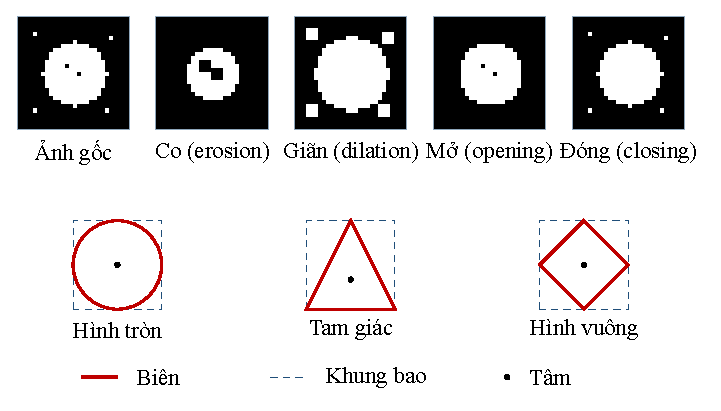
\includegraphics[width=\textwidth]{figures/fig_1_4_morphology_shapes.pdf}
\caption[Phép hình thái học và đặc trưng hình dạng]{Phép co, giãn, mở, đóng trên ảnh nhị phân tự tạo với kernel vuông $3\times3$; bên dưới minh hoạ biên, khung bao và tâm của các hình cơ bản.}
\label{fig:morphology_shapes}
\end{figure}

\subsection{Biến đổi ảnh trong miền tần số}
Trong miền không gian, ảnh được mô tả bằng cường độ tại các vị trí. Trong miền tần số, ảnh được biểu diễn qua các thành phần biến thiên chậm hoặc nhanh. Vùng nền tương đối đồng đều chủ yếu đóng góp vào tần số thấp, còn nét mảnh, đường biên và một phần nhiễu tạo thành phần tần số cao. Bài 2 trình bày hai cách biến đổi thường gặp là Fourier rời rạc và cosin rời rạc~\cite{tailieu_bai2}.

Biến đổi Fourier dùng các thành phần hình sin và cos để mô tả biến thiên theo hai hướng của ảnh. Biên độ thể hiện mức đóng góp của thành phần tần số, còn pha liên quan đến cách các thành phần được sắp xếp trong không gian. Chỉ giữ thông tin biên độ không đủ để tái tạo vị trí chi tiết ban đầu.

Biến đổi cosin rời rạc, thường viết tắt là DCT, biểu diễn ảnh bằng tổng các mẫu cosin. Với nhiều ảnh tự nhiên, phần lớn năng lượng có thể tập trung vào một nhóm hệ số tần số thấp. Điều này cho phép tạo một biểu diễn gọn về cấu trúc tổng thể. Nếu bỏ các hệ số tần số cao, những nét nhỏ cũng có thể bị mất; vì vậy cách rút gọn này không phù hợp để bảo toàn mọi ký tự.

Miền tần số giải thích đánh đổi khi làm trơn: giảm biến thiên nhanh có thể giảm nhiễu nhưng đồng thời làm yếu biên. Tuy nhiên, không thể coi mọi tần số cao là nhiễu và mọi tần số thấp là thông tin cần giữ. Trong so sánh ảnh gần trùng, các thành phần thấp có thể làm dấu hiệu về bố cục chung; trong nhận dạng ký hiệu, chính những nét nhỏ lại có thể quyết định sự khác nhau giữa hai lớp. Cách sử dụng phụ thuộc mục đích của biểu diễn.

\section{Đặc trưng ảnh và giảm chiều dữ liệu}
\label{sec:image_features}
\subsection{Màu sắc, hình dạng và kết cấu}
Đặc trưng chuyển vùng ảnh thành một tập giá trị có cùng quy ước để các mẫu được so sánh hoặc đưa vào mô hình. Đặc trưng màu mô tả phân bố màu; đặc trưng hình dạng mô tả đường bao hay vùng; đặc trưng kết cấu mô tả cách cường độ thay đổi trong một lân cận. Bài 3 phân biệt những thông tin trực tiếp từ điểm ảnh với biểu diễn được tổng hợp trên phạm vi rộng hơn~\cite{tailieu_bai3}.

Tỉ lệ điểm ảnh thuộc một khoảng màu là một đặc trưng đơn giản, ít phụ thuộc kích thước vùng hơn số điểm ảnh tuyệt đối. Tuy nhiên, tỉ lệ đó không cho biết màu nằm ở viền hay ở giữa. Histogram màu cũng bỏ qua nhiều thông tin vị trí. Hai vật thể có cách sắp xếp màu khác nhau vẫn có thể cho biểu diễn gần nhau, nên thường cần thêm thông tin hình dạng hoặc cấu trúc nét.

Đặc trưng cục bộ mô tả một vùng nhỏ quanh điểm nổi bật; đặc trưng toàn vùng tổng hợp cả vùng quan tâm. Các mô tả điểm ở Bài 4 minh hoạ nhu cầu giữ thông tin khi đối tượng thay đổi tỉ lệ hoặc hướng nhìn~\cite{tailieu_bai4}. Lựa chọn giữa hai kiểu mô tả phụ thuộc nhiệm vụ: một vùng rất nhỏ có thể không có đủ điểm nổi bật ổn định, còn một vector toàn vùng lại nhạy với phần nền bị cắt vào.

Khi ghép nhiều loại đặc trưng, cần giữ đúng thứ tự và cách tính ở cả bước học lẫn bước sử dụng. Một giá trị thiếu do không tìm được đường bao phải được phân biệt với giá trị đo bằng 0. Các bước đổi kích thước vùng, chọn mặt nạ và chuẩn hoá cũng là một phần của biểu diễn, vì thay chúng có thể làm vector đầu vào khác với dữ liệu mà mô hình đã học.

\subsection{Mô tả hướng biên}
Bộ mô tả hướng biên HOG thống kê cách các nét phân bố trong vùng ảnh. Thay vì ghi chính xác cường độ của từng điểm, nó gom các hướng biến thiên vào những ô nhỏ. Hai vùng có mức sáng khác nhau nhưng cấu trúc nét gần giống nhau có thể nhận được biểu diễn gần nhau hơn so với việc so trực tiếp từng điểm ảnh~\cite{tailieu_bai5,dalal2005hog}.

Quá trình trích đặc trưng bắt đầu từ một vùng có kích thước thống nhất. Tại mỗi điểm, đạo hàm theo hai hướng được dùng để tính độ lớn và góc theo~\eqref{eq:gradient_magnitude}. Trong mỗi ô, các điểm đóng góp vào histogram hướng, thường có trọng số theo độ lớn. Với biểu diễn không phân biệt dấu, hai hướng chênh $180^\circ$ được gộp lại vì chúng mô tả cùng một phương của nét.

Các ô lân cận được ghép thành khối và chuẩn hoá. Nếu chỉ nhân độ sáng của ảnh với một hệ số, các độ lớn gradient có xu hướng cùng tăng; chuẩn hoá theo khối làm giảm ảnh hưởng của sự thay đổi đó. Các khối có thể chồng lấn để cùng một vị trí được xem trong nhiều lân cận, sau đó các vector khối được nối theo thứ tự cố định~\cite{skimage_hog}.

Có thể hình dung một ví dụ gồm $4\times4$ ô, mỗi ô có 9 khoảng hướng. Nếu mỗi khối gồm $2\times2$ ô và dịch từng ô một, ta có $3\times3$ khối. Mỗi khối có $2\times2\times9=36$ giá trị, nên vector cuối có $3\times3\times36=324$ thành phần. Đây là ví dụ cách xác định số chiều, không phải một kích thước bắt buộc của HOG.

Ô nhỏ mô tả nét chi tiết hơn nhưng nhạy với nhiễu và làm vector dài hơn. Ô lớn tạo biểu diễn gọn hơn nhưng có thể trộn các nét cần phân biệt. HOG cũng không tự bất biến trước mọi phép quay hoặc biến dạng phối cảnh. Chất lượng vùng cắt và lượng chi tiết của ảnh vẫn quyết định thông tin còn lại trong vector.

\subsection{Phân tích thành phần chính}
Phân tích thành phần chính (Principal Component Analysis -- PCA) tìm một hệ trục mới để biểu diễn dữ liệu bằng ít chiều hơn. Những chiều ban đầu có thể chứa thông tin liên quan nhau; giữ tất cả làm tăng bộ nhớ và chi phí tính toán. PCA chọn các hướng có phương sai lớn để giữ phần biến thiên chủ yếu của tập dữ liệu~\cite{tailieu_bai8}.

Giả sử có $n$ vector $\mathbf{x}_i\in\mathbb{R}^{d}$. Trước hết tính vector trung bình $\boldsymbol{\mu}$ và ma trận hiệp phương sai $S$:
\begin{equation}
 \boldsymbol{\mu}=\frac{1}{n}\sum_{i=1}^{n}\mathbf{x}_i,\qquad
 S=\frac{1}{n-1}\sum_{i=1}^{n}(\mathbf{x}_i-\boldsymbol{\mu})(\mathbf{x}_i-\boldsymbol{\mu})^{\top},
 \label{eq:pca_covariance}
\end{equation}
với $n>1$. Các vector riêng trực chuẩn của $S$ xác định những hướng mới; trị riêng cho biết phương sai theo từng hướng. Sau khi sắp theo trị riêng giảm dần, chọn $r<d$ hướng đầu thành các cột của ma trận $U_r\in\mathbb{R}^{d\times r}$. Vector trong không gian giảm chiều là:
\begin{equation}
 \mathbf{z}_i=U_r^{\top}(\mathbf{x}_i-\boldsymbol{\mu}).
 \label{eq:pca_projection}
\end{equation}
Như vậy, $d$ giá trị ban đầu được thay bằng $r$ toạ độ mới; đây là tổ hợp của các đặc trưng cũ, không đơn thuần là xoá một số vị trí trong vector.

Số chiều giữ lại có thể được chọn theo tỉ lệ tổng phương sai hoặc kiểm tra theo nhiệm vụ sử dụng. Giữ nhiều chiều bảo toàn thêm biến thiên nhưng giảm ít chi phí. Giữ quá ít có thể làm mất những nét phân biệt quan trọng. PCA không dùng nhãn lớp để chọn hướng, nên phương sai lớn không đồng nghĩa với khả năng phân loại tốt.

PCA cần trừ trung bình; việc có chuẩn hoá từng đặc trưng về cùng thang đo trước đó hay không là một lựa chọn riêng. Ví dụ, ghép chu vi tính bằng điểm ảnh với tỉ lệ màu trong khoảng 0 đến 1 có thể khiến nhóm giá trị lớn ảnh hưởng mạnh hơn nếu không xử lý thang đo. Tài liệu scikit-learn cũng phân biệt việc trừ trung bình với việc chia theo độ lệch chuẩn~\cite{sklearn_pca}.

Vector trung bình, phép chuẩn hoá và các trục PCA phải được học trên phần huấn luyện thích hợp rồi giữ cố định khi biến đổi dữ liệu xác thực, kiểm thử hoặc ảnh mới. Nếu tính lại trên toàn bộ dữ liệu trước khi chia, thông tin của tập kiểm thử đã ảnh hưởng tới biểu diễn. Cùng một bộ trích đặc trưng nhưng khác bộ PCA cũng tạo ra không gian đầu vào khác nhau.

\subsection{Độ tương đồng và ảnh gần trùng}
So sánh ảnh thường được thực hiện thông qua biểu diễn của chúng. Bài 6 giới thiệu việc dùng khoảng cách giữa các vector để tìm những mô tả gần nhau~\cite{tailieu_bai6}. Khoảng cách nhỏ chỉ có ý nghĩa trong quy ước đặc trưng đã chọn: gần nhau về màu không nhất thiết là cùng đối tượng, còn gần nhau về hình dạng chưa chắc có cùng nội dung chữ.

Hai tệp có thể khác dữ liệu lưu nhưng vẫn cho những ảnh nhìn gần giống nhau, chẳng hạn một ảnh được nén lại hoặc đổi kích thước. Ngược lại, hai ảnh khác cảnh có thể cùng chứa một loại biển. Cần phân biệt trùng tệp, gần trùng về nội dung ảnh và giống nhau về lớp đối tượng, vì chúng phục vụ các mục đích kiểm tra khác nhau.

Mã băm cảm nhận tạo một chuỗi bit ngắn mô tả những dấu hiệu tổng thể của ảnh. Một cách tạo mã là chuyển ảnh về xám, đổi về kích thước thống nhất, tính DCT, lấy một vùng hệ số tần số thấp rồi so với giá trị trung vị để tạo bit~\cite{imagehash_phash}. Đây là ứng dụng của biểu diễn tần số để so sánh bố cục, không phải mã hoá bảo mật hoặc phương pháp đọc nội dung biển.

Với hai mã $h^{(1)},h^{(2)}$ cùng có $L$ bit, khoảng cách Hamming là số vị trí khác nhau:
\begin{equation}
 d_H(h^{(1)},h^{(2)})=\sum_{j=1}^{L}\mathbf{1}[h_j^{(1)}\ne h_j^{(2)}].
 \label{eq:hamming_hash}
\end{equation}
Ký hiệu $\mathbf{1}$ bằng 1 khi điều kiện đúng và bằng 0 khi sai. Khoảng cách nhỏ gợi ý hai biểu diễn giống nhau hơn. Ngưỡng quá rộng có thể gộp nhầm những cảnh khác; ngưỡng quá chặt có thể bỏ qua các bản gần trùng. Ảnh bị cắt nhiều, quay mạnh hoặc có bố cục thay đổi cũng có thể cho mã khác dù cùng nguồn.

Kiểm tra gần trùng giúp hạn chế thông tin lặp giữa các tập dữ liệu. Các nhóm nghi ngờ cần được duyệt cùng nguồn ghi hình trước khi chia tập. Trong một cụm ghép nối tiếp, hai ảnh ở hai đầu vẫn có thể khác nhau đáng kể.


% ==============================================================================
\section{Các nghiên cứu liên quan}
\label{sec:related_work}

Mục này tổng hợp các công trình về nhận diện biển báo theo bốn nhóm: bộ dữ liệu và cách đánh giá, phương pháp truyền thống, phương pháp học sâu cho biển nhỏ, theo vết và xác minh trên video. Mọi tài liệu đã được đối chiếu với nơi công bố (DOI hoặc trang của nhà xuất bản). Số liệu của các công trình khác dùng tập dữ liệu, cách chia và chỉ số khác với đề tài, nên chỉ dùng làm bối cảnh, không so sánh trực tiếp.

\subsection{Bộ dữ liệu và cách đánh giá}
\label{sec:rw_data}

Hai bộ dữ liệu của Đức tách bài toán thành hai phần. GTSRB là bài toán phân loại vùng biển đã cắt sẵn với 43 lớp; trong cuộc thi, một tổ hợp mạng tích chập đạt tỉ lệ phân loại đúng cao hơn người tham gia thử nghiệm~\cite{stallkamp2012gtsrb}. GTSDB là bài toán phát hiện trên ảnh đường phố (900 ảnh, 600 để huấn luyện và 300 để đánh giá), đánh giá riêng theo nhóm biển cấm, nguy hiểm và hiệu lệnh~\cite{houben2013gtsdb}. Việc tách hai phần cho thấy độ chính xác phân loại trên vùng đã cắt không thay thế được chỉ số phát hiện trên cả ảnh. Đề tài áp dụng nguyên tắc này khi so sánh phương pháp truyền thống với YOLO (Mục~\ref{sec:e8}).

Tsinghua-Tencent 100K (TT100K) có 100 nghìn ảnh toàn cảnh với khoảng 30 nghìn biển, phần lớn chiếm diện tích rất nhỏ trong ảnh. Các tác giả chỉ ra rằng mạng phát hiện thiết kế cho vật thể lớn hoạt động kém với biển nhỏ~\cite{zhu2016tt100k}. Bộ dữ liệu Mapillary mở rộng phạm vi ra toàn cầu, có lớp \textit{other-sign} cho biển nằm ngoài danh mục và báo cáo kết quả theo kích thước biển~\cite{ertler2020mapillary}. Đây là tiền lệ cho lớp ``Biển báo khác'' và cho cách phân tích theo kích thước của đề tài.

Với biển báo Việt Nam, Zalo AI Challenge 2020 cung cấp ảnh đường phố độ phân giải $1622\times626$ có nhiều biển rất nhỏ~\cite{zalo2020tsd}; ảnh cùng độ phân giải này chiếm 41\% bộ dữ liệu của đề tài. Pham và cộng sự xây dựng mô-đun nhận diện dựa trên YOLOv5, huấn luyện trên dữ liệu tự thu ngoài đường và chạy trên thiết bị Jetson~\cite{tung2024vietnam}. Cu và cộng sự xây dựng bộ dữ liệu biển nguy hiểm và cảnh báo theo QCVN~41:2019 và dùng YOLOv5 để phát hiện~\cite{cu2024vietnamese,qcvn41_2019}. Các công trình này dùng bộ dữ liệu riêng và chưa so sánh với phương pháp truyền thống trên cùng tập kiểm thử.

\subsection{Phương pháp thị giác máy tính truyền thống}
\label{sec:rw_classic}

Hướng kinh điển gồm hai bước: tìm vùng ứng viên theo màu và hình dạng, sau đó nhận dạng vùng đó. De la Escalera và cộng sự định vị biển bằng ngưỡng màu và hình dạng rồi nhận dạng bằng mạng nơ-ron~\cite{escalera1997road}. Maldonado-Bascón và cộng sự dùng ba giai đoạn: phân đoạn màu, phân loại hình dạng bằng SVM tuyến tính và nhận dạng nội dung bằng SVM nhân Gauss~\cite{maldonado2007svm}. Ưu điểm của hướng này là nhanh và dễ giải thích; nhược điểm là ngưỡng màu thay đổi theo ánh sáng và hình dạng bị biến dạng theo góc nhìn.

HOG mô tả hình dạng bằng histogram hướng gradient trên lưới ô và chuẩn hoá theo khối~\cite{dalal2005hog}. Trên GTSDB, HOG kết hợp bộ phân loại tuyến tính là một trong các phương pháp cơ sở~\cite{houben2013gtsdb}. Vieira so sánh các bước tiền xử lý cho HOG-SVM trên GTSRB: độ chính xác tăng từ 89,65\% lên 91,25\% khi chuyển sang không gian YUV, còn ghép nhiều bước (CLAHE, kênh Hue, YUV) không phải lúc nào cũng tốt hơn~\cite{vieira2025hogsvm}. Đặc trưng điểm khoá như SIFT~\cite{lowe2004sift} kết hợp túi từ thị giác~\cite{csurka2004bovw} hiệu quả với vật thể giàu kết cấu; biển báo lại có ít điểm đặc trưng, nhất là khi biển nhỏ. Đề tài dùng SIFT làm đối chứng âm để kiểm chứng nhận định này (Mục~\ref{sec:e8}).

\subsection{Học sâu và vấn đề biển nhỏ}
\label{sec:rw_deep}

Bộ phát hiện hai giai đoạn như Faster R-CNN đề xuất vùng rồi phân loại~\cite{ren2015faster}; họ YOLO dự đoán khung và lớp trong một lần truyền, phù hợp xử lý thời gian thực~\cite{redmon2016yolo}. Bài tổng quan của Sapkota và cộng sự hệ thống hoá các phiên bản từ YOLOv1 đến YOLOv12~\cite{sapkota2025yolo}. YOLO11 thay đổi khối trích đặc trưng (C3k2, C2PSA) và có nhiều kích cỡ từ \textit{nano} đến \textit{extra-large}~\cite{khanam2024yolo11,ultralytics_yolo11}. Các mô hình này thường được khởi tạo từ trọng số học trên COCO~\cite{lin2014coco} rồi tinh chỉnh cho bài toán đích.

Biển nhỏ là thách thức chung. Với ảnh độ phân giải cao, SAHI chia ảnh thành các ô chồng lấn, chạy bộ phát hiện trên từng ô rồi gộp kết quả. Chỉ riêng bước suy luận cắt ô đã tăng AP 5,1--6,8 điểm trên VisDrone và xView; khi tinh chỉnh thêm trên ô cắt, mức tăng lên 12,7--14,5 điểm~\cite{akyon2022sahi}. Lời giải của nhiều đội tại Zalo AI 2020 cũng dùng cắt ô vì biển rất nhỏ~\cite{zalo2020tsd}. Đề tài không thể bổ sung dữ liệu, nên chỉ thử những cách không cần huấn luyện lại: tăng độ phân giải suy luận và cắt ô khi suy luận (Mục~\ref{sec:t3}).

\subsection{Theo vết và xác minh trên video}
\label{sec:rw_video}

SORT kết hợp bộ lọc Kalman~\cite{kalman1960filter} để dự đoán vị trí và thuật toán Hungarian~\cite{kuhn1955hungarian} để ghép phát hiện theo IoU. Phương pháp rất đơn giản nhưng đạt độ chính xác tương đương các bộ theo vết trực tuyến cùng thời và chạy khoảng 260 khung hình mỗi giây; tác giả cũng nhận xét chất lượng theo vết phụ thuộc nhiều vào bộ phát hiện~\cite{bewley2016sort}. Với biển báo, Šegvić và cộng sự xây dựng chuỗi phát hiện nhất quán theo thời gian rồi lọc chuỗi bằng một mô hình phân biệt học riêng~\cite{segvic2014temporal}. Đây là cơ sở cho thiết kế theo vết và bộ xác minh trong hệ thống của nhóm.

\subsection{Tổng hợp và khoảng trống}
\label{sec:rw_gap}

Bảng~\ref{tab:related_work} tóm tắt các công trình chính và vai trò của chúng trong đề tài.

\begin{table}[H]
\centering
\caption{Tóm tắt các nghiên cứu liên quan}
\label{tab:related_work}
\small
\begin{tabularx}{\textwidth}{|>{\raggedright\arraybackslash}p{3.3cm}|>{\centering\arraybackslash}p{1.2cm}|>{\raggedright\arraybackslash}X|>{\raggedright\arraybackslash}p{4.1cm}|}
\toprule
\textbf{Công trình} & \textbf{Năm} & \textbf{Nội dung chính} & \textbf{Vai trò trong đề tài} \\
\midrule
De la Escalera và cs.~\cite{escalera1997road} & 1997 & Định vị theo màu + hình dạng, nhận dạng bằng mạng nơ-ron & Cơ sở của pipeline CV đối chứng \\ \hline
Maldonado-Bascón và cs.~\cite{maldonado2007svm} & 2007 & Phân đoạn màu, SVM cho hình dạng và nội dung & Cơ sở dùng SVM sau ứng viên màu \\ \hline
Dalal, Triggs~\cite{dalal2005hog} & 2005 & Đặc trưng HOG & Đặc trưng thủ công chính \\ \hline
GTSRB, GTSDB~\cite{stallkamp2012gtsrb,houben2013gtsdb} & 2012, 2013 & Tách đánh giá phân loại và phát hiện & Thiết kế thí nghiệm E8 \\ \hline
TT100K~\cite{zhu2016tt100k} & 2016 & Biển nhỏ trong ảnh toàn cảnh & Phân tích theo kích thước \\ \hline
Mapillary~\cite{ertler2020mapillary} & 2020 & Phạm vi toàn cầu, lớp \textit{other-sign} & Lớp ``Biển báo khác'' \\ \hline
SAHI~\cite{akyon2022sahi} & 2022 & Suy luận và tinh chỉnh trên ô cắt & Thí nghiệm T3 \\ \hline
SORT~\cite{bewley2016sort} & 2016 & Kalman + Hungarian theo IoU & Mô-đun theo vết \\ \hline
Šegvić và cs.~\cite{segvic2014temporal} & 2014 & Chuỗi theo vết + bộ lọc phân biệt & Bộ xác minh \\ \hline
Vieira~\cite{vieira2025hogsvm} & 2025 & Tiền xử lý cho HOG-SVM & Mốc tham chiếu HOG-SVM \\ \hline
Pham và cs.~\cite{tung2024vietnam}; Cu và cs.~\cite{cu2024vietnamese} & 2024 & YOLOv5 cho biển báo Việt Nam & Bối cảnh trong nước \\
\bottomrule
\end{tabularx}
\end{table}

Từ tổng hợp trên, đề tài hướng tới ba vấn đề còn ít được xem xét:
\begin{enumerate}
 \item So sánh trực tiếp phương pháp truyền thống và học sâu trên cùng tập kiểm thử biển báo Việt Nam, theo từng nhóm kích thước biển và có khoảng tin cậy.
 \item Đo đóng góp của từng khâu xử lý ảnh truyền thống trong một hệ thống học sâu, gồm cả những khâu không mang lại cải thiện.
 \item Cải thiện recall biển nhỏ và độ bền với ảnh tối khi không thể bổ sung dữ liệu: tăng độ phân giải suy luận, cắt ô và tăng cường ảnh thích nghi.
\end{enumerate}

